

\begin{frame}{Constructed Exposure Moves Realized Litigation}
\hypertarget{src:firststage}{}
\footnotesize
Regressing the 2020$\to$2024 change in adversarial filings on $\bZ$, with controls and state fixed effects, gives a precise positive coefficient and a cluster-robust effective $F=\HeadlineF$, far above the weak-instrument threshold. Inference uses the $tF$ correction \citep{lee2022}.
\smallskip
\begin{columns}[T]
\begin{column}{0.52\textwidth}
\centering
\resizebox{\linewidth}{!}{% Auto-generated by code/03_estimation/02_iv_main.R
% Do not edit manually -- rerun the generating script to update

\begin{tabular}{l*{4}{c}}
\toprule\toprule
Design: & \textbf{Baseline} & \textbf{Ext.\ controls} & \textbf{Open seats} & \textbf{Contested} \\
\midrule
\rowcolor{mylight}
\textbf{Predicted judicialization} & 0.418$^{***}$ & 0.405$^{***}$ & 0.393$^{***}$ & 0.425$^{***}$ \\
\rowcolor{mylight}
 & \textcolor{mygray}{(0.041)} & \textcolor{mygray}{(0.042)} & \textcolor{mygray}{(0.091)} & \textcolor{mygray}{(0.053)} \\
\midrule
First-stage $F$ & 102.3 & 93.3 & 18.6 & 65.1 \\
$N$ & 5,560 & 5,560 & 2,026 & 3,534 \\
\bottomrule\bottomrule
\end{tabular}
}\\[8pt]
\raggedright\scriptsize Coefficient $\FSCoef$ is the rise in $\Delta\log(1+\text{lawsuits})$ per unit of exposure. It is stable under the full control set (col.\ 2) and reproduces in each seat-type subsample (cols.\ 3--4).
\end{column}
\begin{column}{0.46\textwidth}
\centering
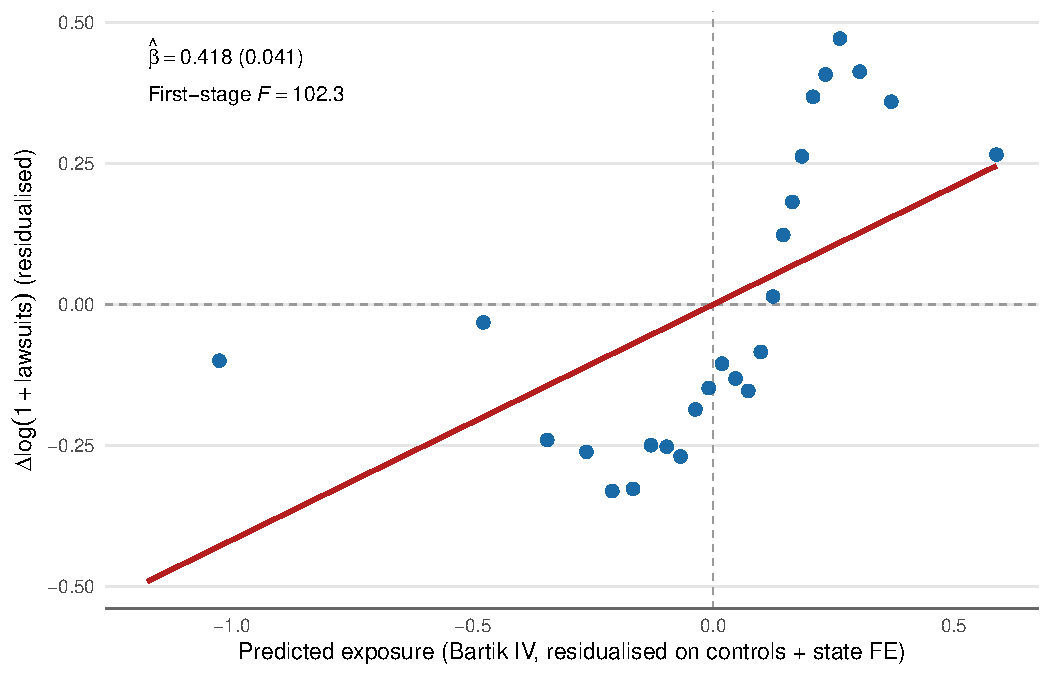
\includegraphics[width=\linewidth,height=0.52\textheight,keepaspectratio]{../figures/firststage_linear.pdf}\\[4pt]
\raggedright\scriptsize Realized growth against predicted exposure, both residualized on controls and state fixed effects (25 equal-count bins). The relationship is a single line through the origin, slope $\hat\beta=\FSCoef$.
\end{column}
\end{columns}
\smallskip
\centerline{\hyperlink{app:extensive}{\beamergotobutton{Zero-vs-any litigation?}}\quad\hyperlink{app:reclass}{\beamergotobutton{A coding artifact?}}}
\end{frame}
